\subsection{Wave-breaking field}
\underline{Dawson's derivation} [Note: The wave-breaking field does not represent the onset of the non-linear regime but the highest achievable field in the non-linear regime.]
We consider a simple 1D linear non-relativistic electron sheet model first used by Dawson \citep{Dawson1959} to show the breakdown of the linear model (\textcolor{red}{correct?}). Consider the plasma being made up of thin sheets of ions and electrons. A sheet at equilibrium position $z=z_0$ is then displaced by $\eta_0(z_0)$, where the displacement is set as function of the equilibrium position for full generality, to a new position $z=z_0+\eta_0$. The displaced sheet reveals a positive surface charge density $\sigma=en_0\eta_0$, where $n_0$ is the electron charge density in the plasma. This sets up a restoring electric field which we find using Gauss's law to be $E_{\text{res}}=4\pi n_0e\eta_0$ which yields a restoring force
\begin{equation}
 m_e\frac{\partial^2\eta_0}{\partial t^2}=-eE_{\text{res}}=-4\pi n_0e^2\eta_0=-\omega_p^2\eta_0
 \end{equation} 
 with solutions 
 \begin{equation}
 \eta_0(z_0,t)=A_1(z_0)\cos(\omega_p t)+A_2(z_0)\sin(\omega_p t)
 \end{equation}
The phenomena of wave breaking can be shown by considering another electron sheet at an equilibrium position $z_1=z_0+\Delta z_0$ at a distance $\Delta z_0$ away from the first sheet. This sheet is then displaced by $\eta_1$ to a new position $z^{*}_1=z_0+\Delta z_0+\eta_1$. The linear model is valid provided that there are no electron trajectories intersect one another in the plasma [ \textcolor{red}{is this correct? Why does the model break down?} ]. Hence the model is valid provided that $z^{*}_1-z_0>z-z_0$ which implies that we must have
\begin{equation}
\Delta z_0+\eta_1>\eta_0~,
\label{eta_ineq}
\end{equation}
for all $\Delta z_0\in \mathbb{R}$, to sustain plasma oscillations in the linear model. We now consider  the limit as $\Delta z_0\to 0$ for the expression 
\begin{equation}
\frac{\partial \eta}{\partial x_0}=\lim_{\Delta z_0\to 0}\frac{\Delta \eta}{\Delta z_0}=\lim_{\Delta z_0\to 0}\left(\frac{\eta_1-\eta_0}{\Delta z_0}\right)>\lim_{\Delta z_0\to 0}\left(\frac{\eta_0-\Delta z_0-\eta_0}{\Delta z_0}\right)=-1
\end{equation}
which simplifies to
\begin{equation}
\frac{\partial \eta}{\partial z_0}>-1
\label{no_crossing}
\end{equation}
where the inequality is introduced using Eq. (\ref{eta_ineq}). We now consider the special case where $A_1(z_0)=A\sin(k_pz_0)$ and $A_2(z_0)=0$. This is a valid solution since $\sin(k_pz_0)$ is single-valued for all $k_p,x_0\in\mathbb{R}$. This particular solution is chosen to highlight the breadown of the electric field, and is motivated by ([\textcolor{red}{what?}]) the solution we found for the electric field in section 2. Applying the no-crossing criterion in Eq. \ref{no_crossing} to $\eta=\eta_0(z_0,t)$ yields
\begin{equation}
\frac{\partial \eta_0}{\partial z_0}=Ak_p\cos(k_pz_0)>-1 \quad \Leftrightarrow \quad Ak_p\leq 1
\end{equation}
which gives the maximum amplitude as $A_{max}=1/k_p$. Hence the maximum restoring electric field $E_{max}\equiv E_{\text{wb}}=4\pi n_0/k_p$ is given by
\begin{equation}
E_{\text{wb}}=\frac{m_ev_p\omega_p}{e}
\end{equation}
the so-called \textit{wave-breaking field}. To further show how this breaks the linear model we consider the effect on the electric field up to and past the wave-breaking limit. As above we have, 
\begin{equation}
z=z_0+\eta_0=z_0+A\sin(k_p z_0)
\label{dawson_z}
\end{equation}
and 
\begin{equation}
E=4\pi n_0e A\sin(k_p z_0)
\label{dawson_E(z)}
\end{equation}
from which we want to find the electric field as a function of $z$. We can do this by numerically solving Eq. \ref{dawson_z} for $z_0$ in a range of $z$ values given fixed values of $A$. The gives $z_0=z_0(z,A)$ which can be substituted into Eq. \ref{dawson_E(z)} to give $E=E(z,A)$, the result of which is shown in Fig. \ref{DawsonCriterionPlot}. From this we conclude that the electric field is no longer single-valued for $A>1/k_p$, i.e past the electric field's wave-breaking amplitude, which signifies a breakdown of the linear model.\\
This is further emphasized by consider the electron-density response as $\partial \eta/\partial z_0\to -1$. To do this we use  Eq. XXX in 1D with no beam density $n_b=0$, 
\begin{equation}
\frac{\partial E}{\partial z}=4\pi e(n_0-n)
\end{equation}
where $n=n_0+n_1$ is the perturbed plasma density and $n_0$ is the ion density, hence $n_0-n$ is the free (negative) charge density in the plasma. We now take the derivative of the perturbed electric field and substitute the above expression
\begin{equation}
\frac{\partial E}{\partial z}=4\pi n_0 e \frac{\partial \eta}{\partial z} \quad \Rightarrow \quad n=n_0\left(1-\frac{\partial \eta}{\partial z}\right)
\end{equation}
We now rewrite $\partial /\partial z$, using $z=z_0+\eta$, as
\begin{equation}
\frac{\partial}{\partial z}=\left(1-\frac{\partial \eta }{\partial z_0}\right)^{-1}\frac{\partial}{\partial z_0}
\end{equation}
which gives
\begin{equation}
n=\frac{n_0}{1+\frac{\partial \eta }{\partial z_0}}
 \end{equation} 
 which means that the perturbed electron density grows infinite as $\partial \eta/\partial z_0\to -1$, again signifying the breakdown of the linear model.\\
\\
Having seen that the linear theory can break down mathematically, it is crucial to ask whether this is realised in 3D models and experiments as well. 
\begin{figure}
\centering
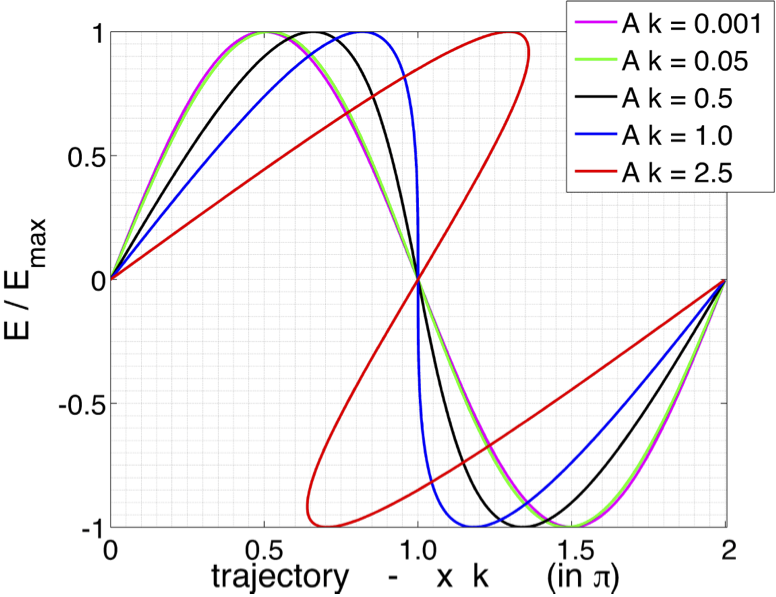
\includegraphics[scale=1]{SahaiThesisPlot.png}
\caption{Plot corresponding to Dawson's derivation of the wave-breaking field [ref. Sahai].}
\label{DawsonCriterionPlot}
\end{figure}

\clearpage
\section{Particle interactions with matter}
Conventional beam dumps work by stochastic interactions of the beam with the dense medium [hanahoe 6.5]
\subsection{Bohr-Fermi-Bethe-Bloch Theory}
Bethe-Bloch forumla:
\begin{equation}
-\expval{\frac{\mathrm{d}U}{\mathrm{d}s}}_{\text{ion}}=\frac{4\pi e^4n_{e,m}}{m_ec^2\beta^2}\left[\ln\left(\frac{2m_e\gamma^2v^2}{I}\right) -\beta^2\right]
\end{equation}

\subsection{Collective Plasma Deceleration -- Non-Linear regime }
\clearpage
\begin{figure}
\centering
\includegraphics[width=1.15\textwidth]{visit0098.pdf}
\caption{Non-linear regime, plasma density perturbations. Added custom legend with density=number of electrons / grid-square size. }
\end{figure}

\begin{figure}
\centering
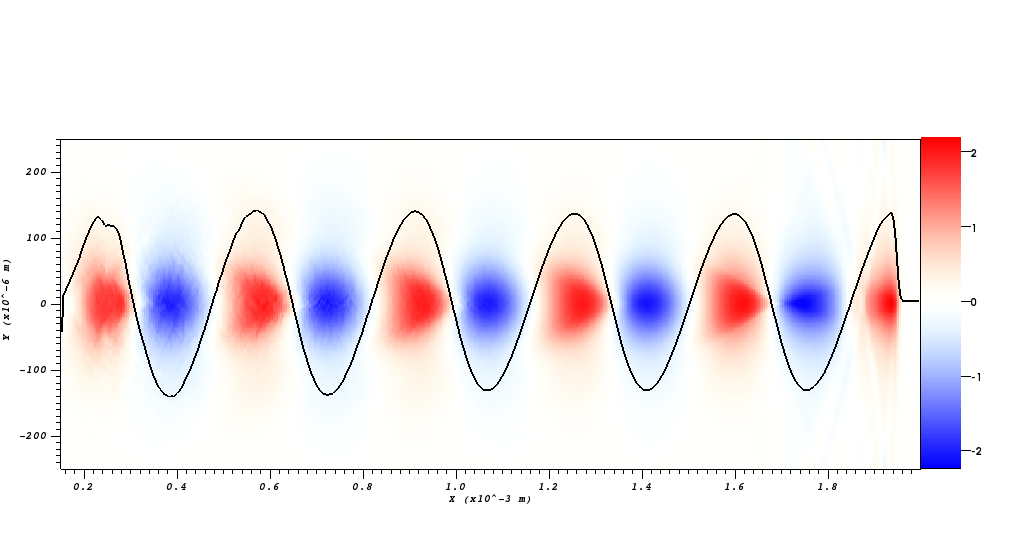
\includegraphics[width=\textwidth]{Ex_nonlinear.png}
\end{figure}
\begin{figure}
\centering
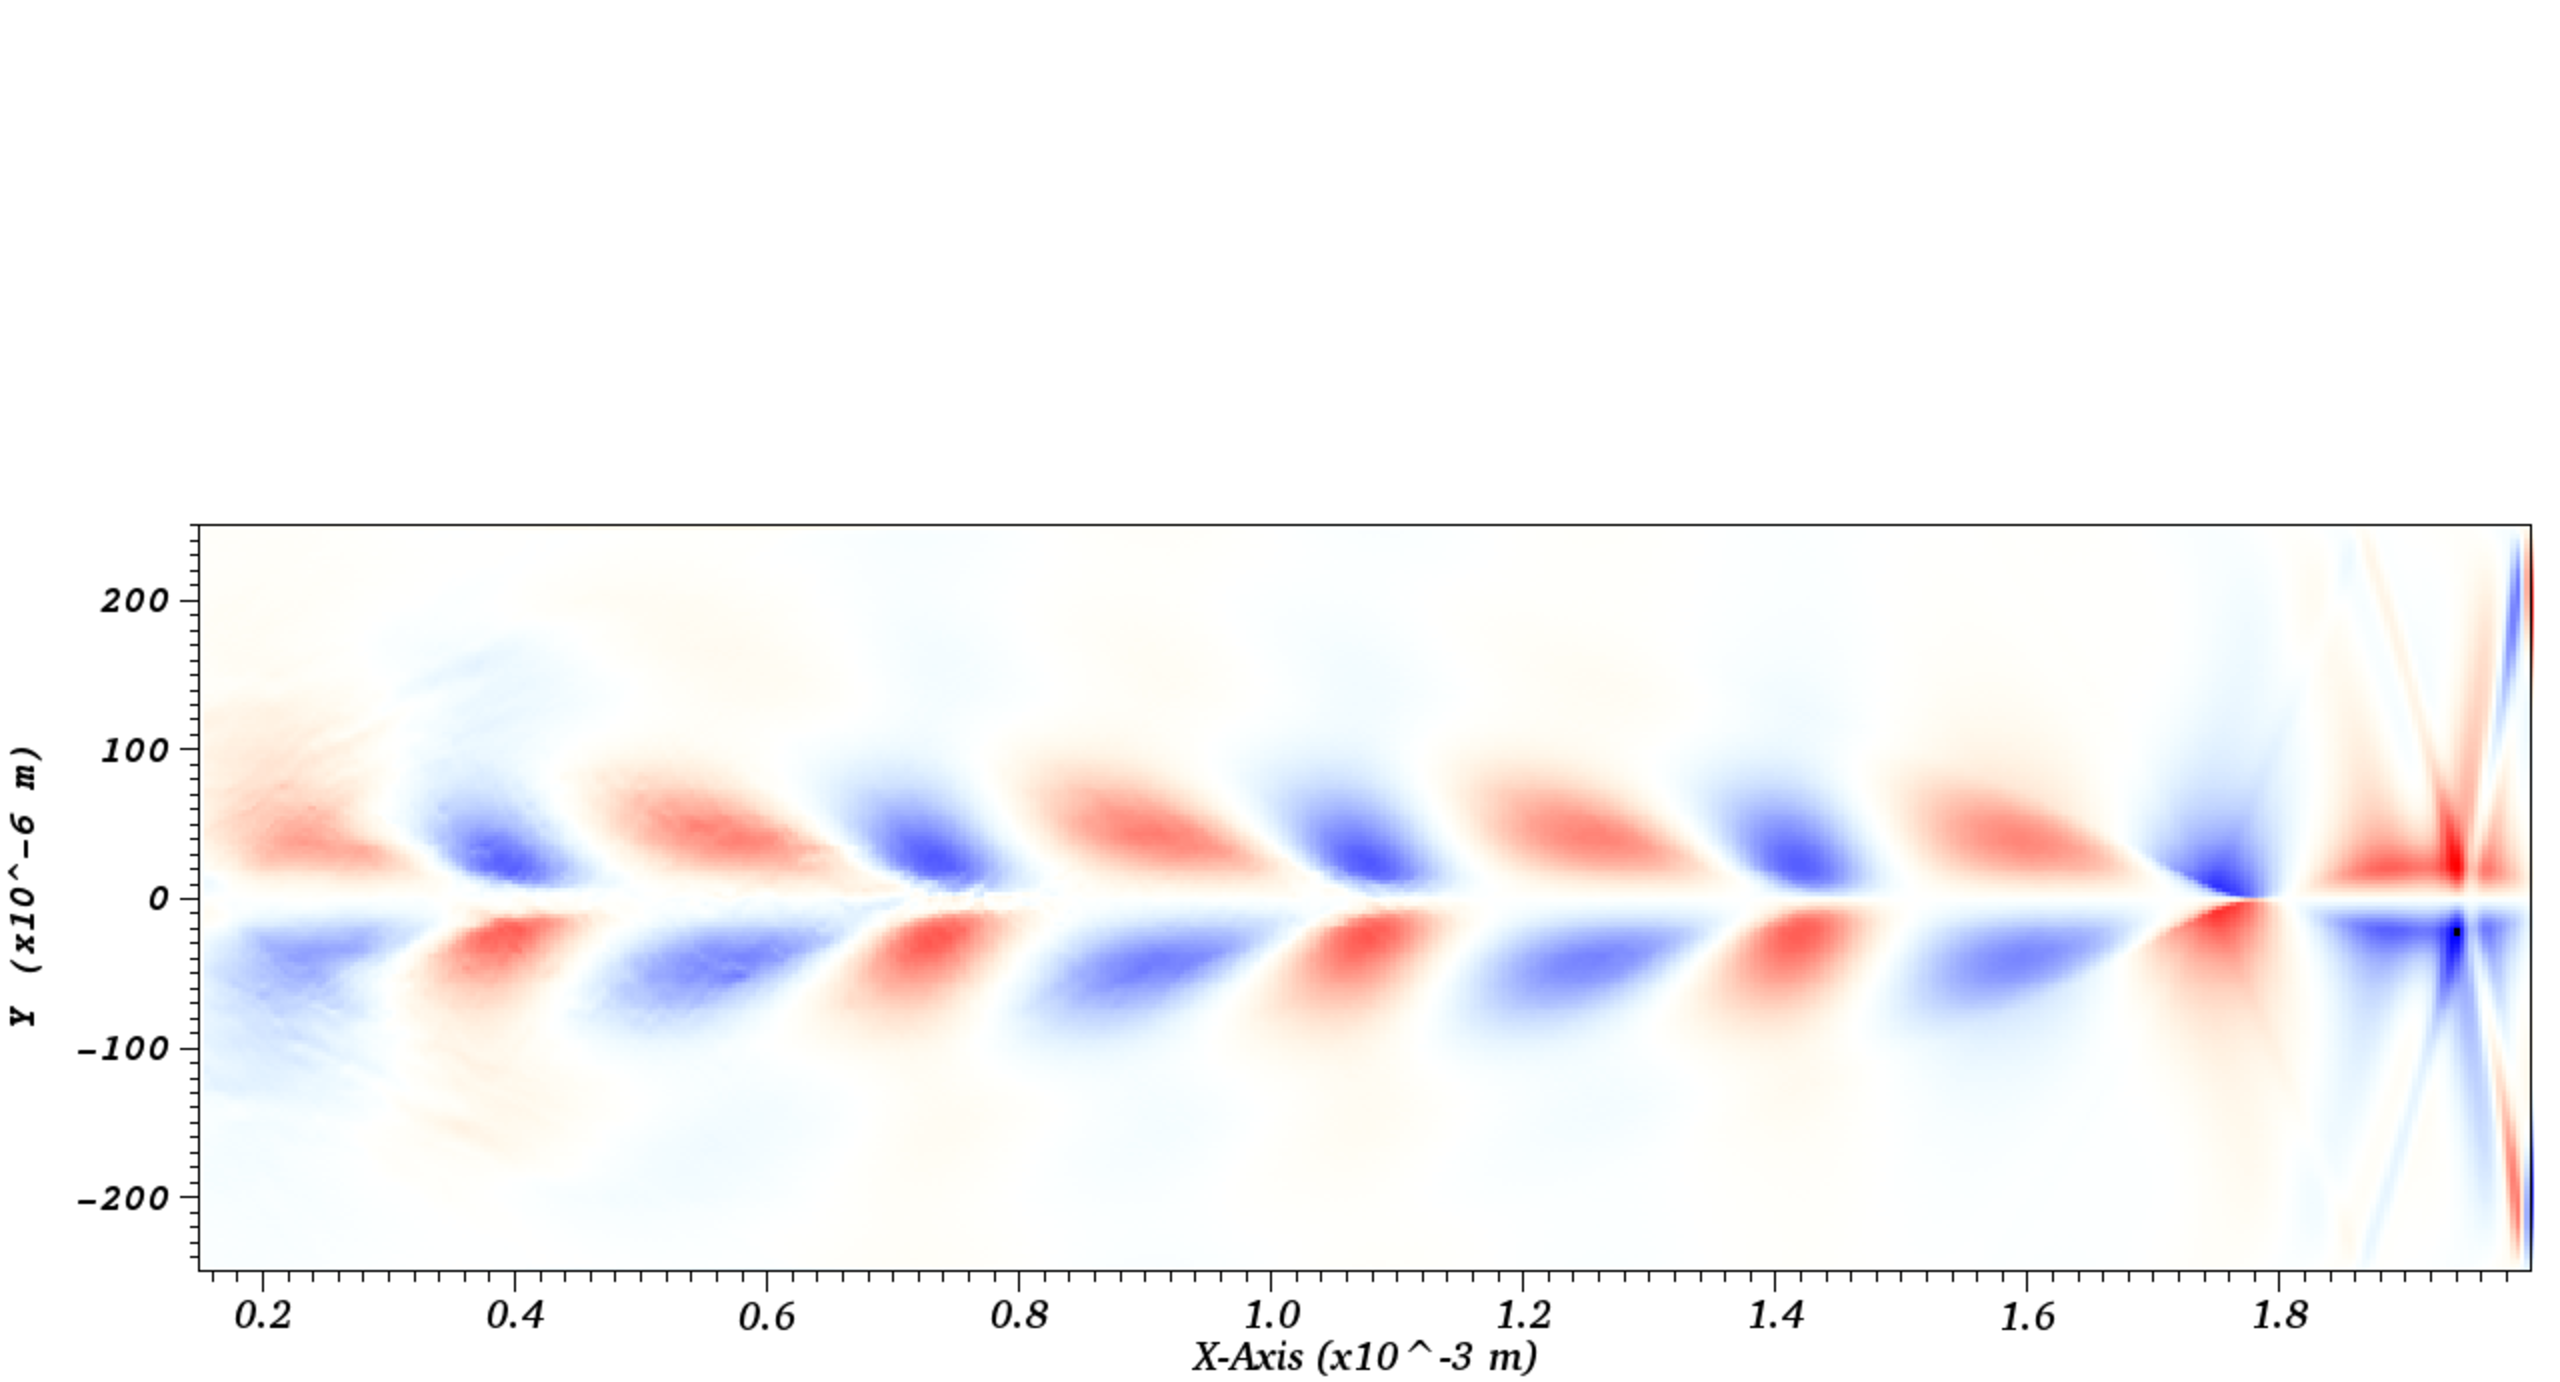
\includegraphics[width=\textwidth]{Ey_nonlinear.png}
\caption{Should these three plots be in results or here? OR PUT SIMUALTIONS CHAPTER BEFORE THEORY CHAPTER. Then theory can be used to also verify that simulations work. Probably not, better explain everything to motivate what simulations to be done }
\end{figure}
\begin{equation}
-\left(\frac{\mathrm{d}E}{\mathrm{d}z}\right)_{\text{coll-wave-break}}=F_e=eE_{wave-break}=m_e c\omega_{p}\left(\frac{n_b}{n_e}\right)
\end{equation}

What is the wave-breaking electric field?

\section{Notes.}
Meeting Guoxing:
\begin{itemize}
\item We will change $\sigma_{x,y}$, in simulation from $\sigma_{x,y}=0.3 \mu m ~\to~5-10 \mu m$ because the $0.3\mu m$ EuPRAXIA beam parameter gives to high beam density $n_b$, which means that we can't have $n_b\sim n_p$ because the plasma density would have to be too high. We should aim for $n_p\sim 10^{17}-10^{18}\sim n_b$ (standard L/PWFA) parameters. 
EuPRAXIA wants $\sigma_{x,y}$ small because small bunches gives more coherent radiation in undulators. One could expand the beam by letting it propagate freely (expand due to space charge) a distance before reaching the beam dump. 
\item $\text{Run simulations with uniform plasma density for }\left\{\begin{aligned}
&n_p\sim 0.1 n_b \quad &&\text{Non-linear}\\
&n_p\sim  n_b\quad &&\text{Quasi-linear}\\
&n_p\sim 10 n_b\quad &&\text{Linear}
\end{aligned}\right.$ \\
\item Use $\Delta E/E=0.01$ and bunch charge $30~$pC ($5~$fs).\\
\item Estimate necessary simulation propagation length by saturation length using wave-breaking electric field gradient 
$$L_{\text{sat}}\approx \frac{T_0}{eE_{wb}}=\frac{T_0}{e}\frac{e}{m_e c\omega_p}=\frac{T_0}{m_e c}\sqrt{\frac{m_e e\epsilon_0}{e^2n_b}} $$ 
\item Project outline:
\begin{itemize}
\item Uniform plasma with varying $n_b\sim n_p$
\item Vary plasma density profile
\item Test laser to dump head of beam
\item Run simulations for real FlashForward parameters and not the idealized EuPRAXIA parameters.
\end{itemize}
\item  100pC $$n_b=\frac{N_p}{(2\pi)^{3/2} \sigma_y^2\sigma_x}=\frac{6.25\times 10^{8}}{(2\pi)^{3/2} (5\times 10^{-6})^3}\approx 3.2\times 10^{23}~ \text{m}^{-3} $$
$$\Rightarrow ~~eE_{\text{wb}}=\left\{\begin{aligned}
&17 ~\text{GeV/m }&& n_p=0.1 n_b \\
&54 ~\text{GeV/m} && n_p=n_b\\
&172 ~\text{GeV/m} &&n_p=10 n_b
\end{aligned}\right.\quad\Rightarrow ~~L_{sat}(1 ~\text{GeV})=\left\{\begin{aligned}
&5.8 ~\text{cm}&& n_p=0.1 n_b \\
&1.9 ~\text{cm} && n_p=n_b\\
&0.6 ~\text{cm} &&n_p=10 n_b
\end{aligned}\right.$$
$$1 ~\text{GeV beam} ~~\Rightarrow ~~ L_{sat}\sim 2 ~\text{cm}=2*10^4 \mu \text{m} $$
\item  30pC $$n_b=\frac{N_p}{(2\pi)^{3/2} \sigma_y^2\sigma_x}=\frac{1.87\times 10^{8}}{(2\pi)^{3/2} (5\times 10^{-6})^3}\approx 9.5\times 10^{22}~ \text{m}^{-3} $$
$$\Rightarrow ~~eE_{\text{wb}}=\left\{\begin{aligned}
&9.4 ~\text{GeV/m }&& n_p=0.1 n_b \\
&30 ~\text{GeV/m} && n_p=n_b\\
&94 ~\text{GeV/m} &&n_p=10 n_b
\end{aligned}\right.\quad\Rightarrow ~~L_{sat}(1 ~\text{GeV})=\left\{\begin{aligned}
&10.7 ~\text{cm}&& n_p=0.1 n_b \\
&3.4 ~\text{cm} && n_p=n_b\\
&1.1 ~\text{cm} &&n_p=10 n_b
\end{aligned}\right.$$
$$1 ~\text{GeV beam} ~~\Rightarrow ~~ L_{sat}\sim 3.4 ~\text{cm}=3.4*10^4 \mu \text{m} $$



\clearpage
\begin{verbatim}
ExportDBAtts = ExportDBAttributes()
ExportDBAtts.allTimes = 0
ExportDBAtts.dirname = "/Users/oscarjakobsson/Documents/epoch-4.14.4/epoch2d"
ExportDBAtts.filename = "test"
ExportDBAtts.timeStateFormat = "_%04d"
ExportDBAtts.db_type = "Xmdv"
ExportDBAtts.db_type_fullname = "Xmdv_1.0"
ExportDBAtts.variables = ("Particles/Ek/edriver", "Particles/Weight/edriver")
ExportDBAtts.writeUsingGroups = 0
ExportDBAtts.groupSize = 48
ExportDBAtts.opts.types = (0)
ExportDBAtts.opts.help = ""
ExportDatabase(ExportDBAtts)
ExportDBAtts = ExportDBAttributes()
ExportDBAtts.allTimes = 0
ExportDBAtts.dirname = "/Users/oscarjakobsson/Documents/epoch-4.14.4/epoch2d"
ExportDBAtts.filename = "test"
ExportDBAtts.timeStateFormat = "_%04d"
ExportDBAtts.db_type = "Xmdv"
ExportDBAtts.db_type_fullname = "Xmdv_1.0"
ExportDBAtts.variables = ("Particles/Ek/edriver", "Particles/Weight/edriver")
ExportDBAtts.writeUsingGroups = 0
ExportDBAtts.groupSize = 48
ExportDBAtts.opts.types = (0)
ExportDBAtts.opts.help = ""
ExportDatabase(ExportDBAtts)

\end{verbatim}

\begin{itemize}
\item Issue: restart not possible with laser. 
\item EPOCH allows for a user to manually override particle-parameter distributions defined in the input deck, in which all functions must be defined analytically. By overriding this so-called autoloader, which takes the analytical distributions in the input deck and distributes the macro particles accordingly, this manual approach allows for the initialisation of a bunch with non-analytical density and momentum distributions. 
\item Furthermore, even if the density distribution were to be easily described analytically, this method offers the advantage that it also overrides the maxwellian velocity distribution that epoch assigns to each bunch of particles in the input deck. This is fine for an initial bunch in thermal equilibrium, but as soon as plasma interaction occurs the velocity distribution of the electrons in the bunch is noticeably non-maxwellian
\item VisIt - export data from .sdf file, convert to -csv, read with ic module when compiling epoch.
\item (show below, it is possible to have a laser appear before the bunch at some time t, but the parameters of this laser could not be changed so testing several differnt laser intensities, distances etc. would take far too long if the bunch was forced to propagate 20cm each time before the laser was ramped up )
\end{itemize}

\subsection{Input deck}
Once EPOCH has been downloaded and compiled the so-called input deck is essentially EPOCH's user interface. This is a file in which users specify the details of a simulations and it is this file that gets read by EPOCH and passed onto the core PIC algorithm. The input deck consists of blocks which define parameters for different features of the simulation. \\
\textbf{Explain control block first}, and what the restart does.
\begin{verbatim}
begin:control
  dlb_threshold = 0.5
  restart_snapshot=restartXXXX.sdf
  t_end = end_time
  nx = nint(length / cell_length)
  ny = nint((half_width * 2) / cell_width)
  npart = part_per_cell * nx * ny
  stdout_frequency = 50
  use_random_seed = T
end:control
\end{verbatim}
This specifies the grid that the simulations is to run on. We then populate this grid with plasma particles.
\textbf{Species block}, with explanation about analytical density distributions for plasma, and specify ppc.\\
The control and species blocks together define the resolution of the simulation. When setting up the resolution of the grid one has to make sure that the grid is sufficiently fine such that the smallest features of our physical system are resolved. This is to ensure that the simulation accurately models the physical system it is meant to represent, to the extent that missing small scale phenomena might alter the large scale outcome of the simulation. A finer grid however requires more macroparticles to fully populate the grid, which inevitably extents the computational time. In addition the time step $\Delta t$ aneeds to be suitably decreased as well. This is because of the so-called Courant-Friedrichs-Lewy (CFL) condition.  Any simulation introduces uncertainties in the final outcome due to the finite resolution. We need to make sure that the uncertainties introduces during each iteration do not build up and grow unbounded. \\
\\
\textbf{edriver} with analytical distribution, and laser, followed by boundaries
\begin{center}
\begin{verbatim}
begin:boundaries
  bc_x_min = simple_laser
  bc_x_max = simple_outflow
  bc_y_min = simple_outflow
  bc_y_max = simple_outflow
end:boundaries
\end{verbatim}
\end{center}
\textbf{output block} and the sdf file visualisation with VisIT

%Parameters and initial conditions are defined using an \textit{input.deck} file.

%$$n_b = \frac{1}{{\sigma_x\sigma_y^2 (2\pi)^{3/2 }  }}e^{{{ - \left( {x - x_0 } \right)^2 } \mathord{\left/ {\vphantom {{ - \left( {x - x_0 } \right)^2 } {2\sigma_x ^2 }}} \right. \kern-\nulldelimiterspace} {2\sigma_x^2 }}}e^{{{ - \left( {y - y_0} \right)^2 } \mathord{\left/ {\vphantom {{ - \left( {y- y_0 } \right)^2 } {2\sigma_y ^2 }}} \right. \kern-\nulldelimiterspace} {2\sigma_y ^2 }}}e^{{{ - \left( {y - y_0 } \right)^2 } \mathord{\left/ {\vphantom {{ - \left( {y - y_0 } \right)^2 } {2\sigma ^2 }}} \right. \kern-\nulldelimiterspace} {2\sigma_y ^2 }}}$$